\newacronym{gpu}{GPU}{graphics processing unit}
\newacronym{ik}{IK}{inverse-kinematics}
\newacronym{lbs}{LBS}{linear blend skinning}
\newacronym{ct}{CT}{computed tomography}

In this section the related works will be announced and summarized. The section is segmented topic wise and it also includes previous works of ideas that may not have managed to be implemented in the course of this thesis.

\section{Ultrasound data handling}

From a technical perspective ultrasound is an acoustical investigation and therefore is susceptible of various noise induced artefacts \cite{Solteszova2012}. The ultrasound investigation is somehow limited to the investigation area which is unable to perceive for example the whole liver or also the whole fetus at a glance \cite{Viola2013}. Therefore techniques to generate compund volumes on the fly are important \cite{Viola2013,Muller2014}. 

\subsection{Filtering 3D ultrasound}

Especially when using \gls{3d} ultrasound investigations in a medical context some kind of filtering is essential in order to perceive anatomical structures visually and mentally. Therefore Solteszova et.al. introduced a technique called Lowest-Variance Streamlines for filtering \gls{3d} ultrasound \cite{Solteszova2012}. The filtering identifies borders of structures by calculating the lowest variance direction. According to Solteszova et.al. their procedure is similar to a streamline integration in a vector field. The approach is interesting because it is especially useful for medical ultrasound applications in order to reduce artefacts like noisiness and speckles which may lead to a miss interpretation of the underlying data. The output of the filtering method can be seen in Figure \ref{fig:Streamline}.

\begin{figure} [htb!]
    \centering
	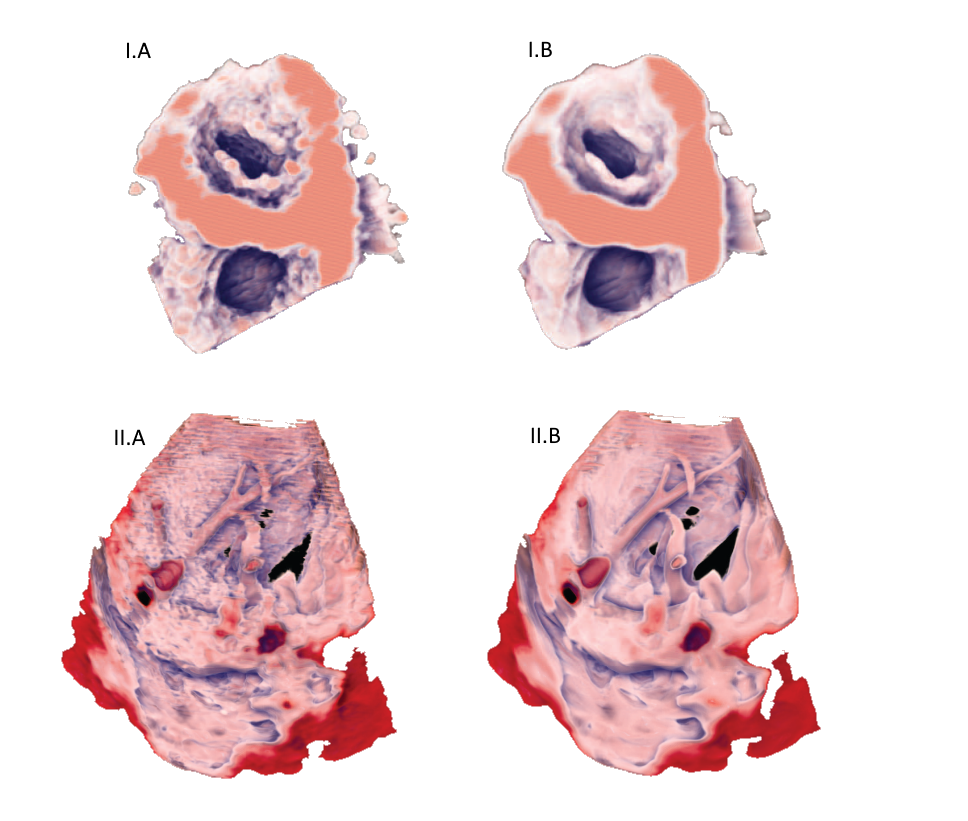
\includegraphics[width=16cm]{content/images/streamline}
	\caption{I.A and I.B depict a cardiac ultrasound before and after filtering and II.A and II.B show an ultrasound of the liver before and after filtering \cite{Solteszova2012}.}
	\label{fig:Streamline}
\end{figure}

\newpage
Solteszova et.al. also introduced another approach for filtering especially fetal ultrasound called the output-sensitive filtering of streaming volume data \cite{Solteszova2017}. The approach is espaccially design to be used in \gls{4d} ultrasound investigations where it is important that the filtering is very fast and accurate. They limit the filtering to regions of the volume which have a potential to have an effect on the image e.g. occluded regions don't have to be filtered because they cannot be seen anyways. They state that their approach is an important improvement for streaming volume data as it is the case in a \gls{4d} ultrasound investigation. The output of the filtering applied to a fetal ultrasound investigation of Anna is depicted in Figure \ref{fig:outputSensitive}.

\begin{figure} [htb!]
    \centering
	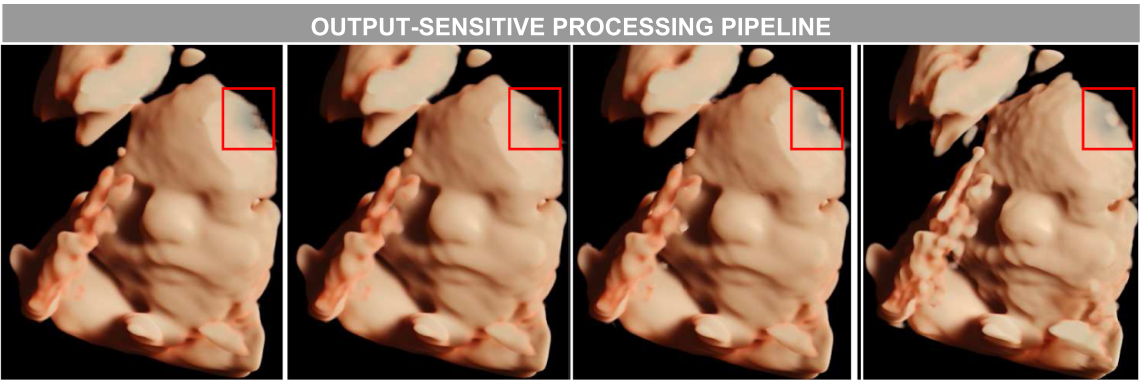
\includegraphics[width=16cm]{content/images/outputSensitive}
	\caption{The output of the otput-sensitive processing pipeline with different percentage amounts of voxels filtered. From 38\% on the left side to 0\% on the right side \cite{Solteszova2017}.}
	\label{fig:outputSensitive}
\end{figure}

\newpage
\subsection{Compound volume generation}

Viola et.al. states that a compound view of volumetric data created by ultrasound investigation can be useful for clinical investigation \cite{Viola2013}. It enables the clinicians to e.g. slice through an whole organ after is has been registered at a glance. Especially in fetal ultrasound investigation after a specific time, when the fetus is too large to be perceived as a whole, registering the data as well as producing a compound-volume is very useful and essentially for the introduced procedure. The possibility to swipe with the ultrasound investigation probe over the body and seeing the result on the screen in real-time producing a compound volume is essential for a better understanding of the examined specimen. The creation of a compound volume presented by Viola et.al. is depicted in Figure \ref{fig:SwipeVol}.

\begin{figure} [htb!]
    \centering
	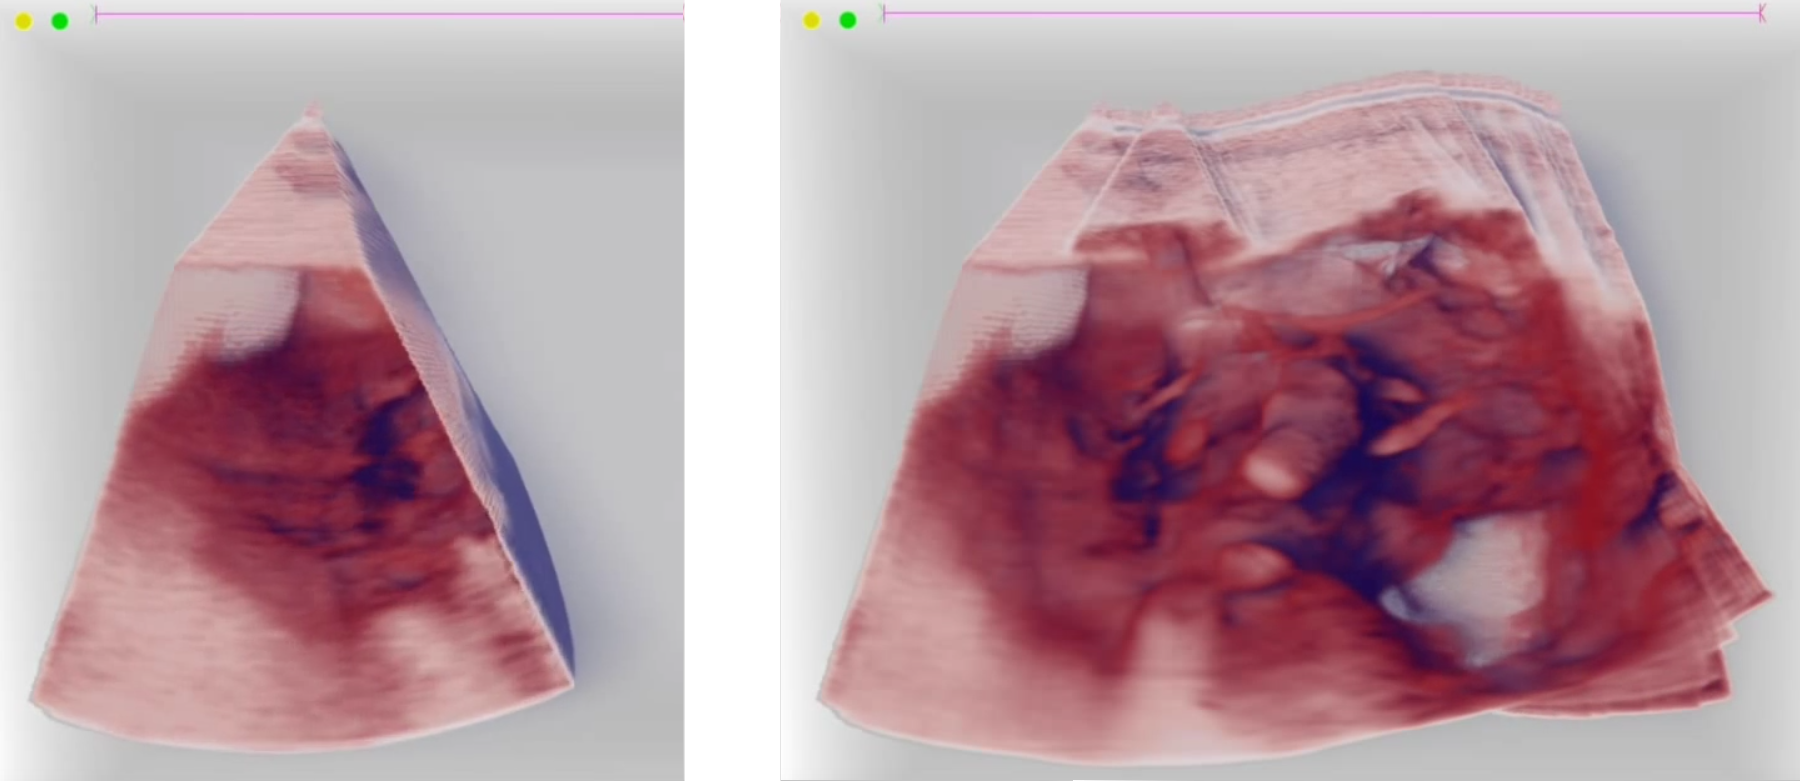
\includegraphics[width=12cm]{content/images/Swipevol}
	\caption{On the fly creation of a compound volume by Viola et.al. The right part of the image in comparison to the left part shows the progress of the compound volume generation. The images have been taken from the video of \cite{Viola2013}.}
	\label{fig:SwipeVol}
\end{figure}

Being able to automatically register and process \gls{4d} ultrasound data without externally tracking the ultrasound probe can be tough \cite{Muller2014}. Mueller et.al. state that their approach of generating a compound volume of the liver uses multi-modal registration considering the \gls{3d} voxel neighbourhood. They have used various transformations and optimization strategies in order to register the different ultrasound investigations during one session. They also had to cope with anatomical distortions of the ultrasound investigation which they stated had not an significant impact if the continuous motion of the investigation sweep had no rapid changes in direction.\newline\newline

\section{Understanding the data}
Having the ultrasound data of the fetal investigation filtered and registered in order to generate the whole volume the next steps will be about figuring out the position of the fetus. There are different approaches to find more detailed content wise information of volumetric data. One step would be to skeletonize the data and try to find out if the joints and bones of the fetus can be found automatically \cite{Singh2004,Jin2017,Jalba2013}. Another approach is to rig the data by include a predefined armature or skeleton which is than either automatically \cite{Baran2007,Baran} or manually \cite{Finet2014Bender:Morphing} included in the data. 

\subsection{Skeletonization}

Skeletonization of data is an approach where it is tried to reduce the given object to the most important features \cite{Singh2004}. This description may then be used for further processing and can be linked back to the data it has been abstracted from \cite{Jalba2013}. When writing about \gls{3d} skeletonization one has to distinguish between surface and curve skeletons. According to Jalba et.al. the surface skeleton of a \gls{3d} shape is the collection which contains the "loci of maximally-inscribed balls in a shape" \cite{Jalba2013, Pizer2003MultiscaleProperties}. In respect to the surface skeleton the curve skeleton may be described as one dimensional curves which are positioned at the center of the \gls{3d} shape. The second skeleton is especially interesting when trying to transform fetus data. Jalba et.al. presented a technique which is based on the \gls{gpu} for calculating curve skeleton points by firstly evaluating the surface skeleton and then detecting the curve skeleton points by their algorithm \cite{Jalba2013}. Their algorithm works fast and reliable and delivers a high-quality curve skeleton and automatically delivers the mapping to the underlying data. The results of their approach are depicted in Figure \ref{fig:CurveSkeleton}.

\begin{figure} [htb!]
    \centering
	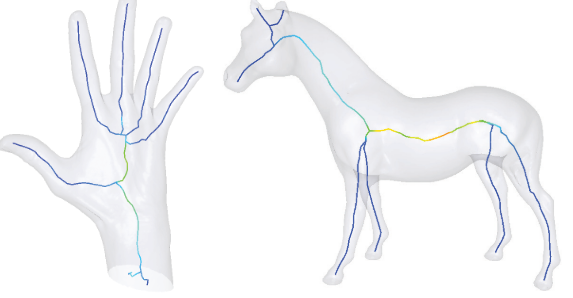
\includegraphics[width=11cm]{content/images/curveSkeletonJalba}
	\caption{Result of the curve skeleton produced by the algorithm introduced by Jalba et. al. for a human hand on the left and a horse on the right \cite{Jalba2013}.}
	\label{fig:CurveSkeleton}
\end{figure}

\newpage
Another approach to produce a skeletal representation of in that case voxel data is presented by Jin and Kim \cite{Jin2017}. Their algorithm is based on a thinning approach and can be implemented on the \gls{gpu}. Jin and Kim identified general patterns of \gls{3d} neighbourhood relation which can be used in order to decide if a voxel is part of the skeleton or not. The algorithm can be executed in parallel for each voxel in the data. They also introduced a skeleton correction algorithm which takes care of connecting skeletal parts which may have been disconnected by the thinning algorithm. The authors evaluated their approach using 100 models of the SHREC 2015 benchmark testing set and state that their proposed algorithm is robust and provides an overall good performance. The results when performing on a human model can be seen in Figure \ref{fig:skeletonThinning}.

\begin{figure} [htb!]
    \centering
	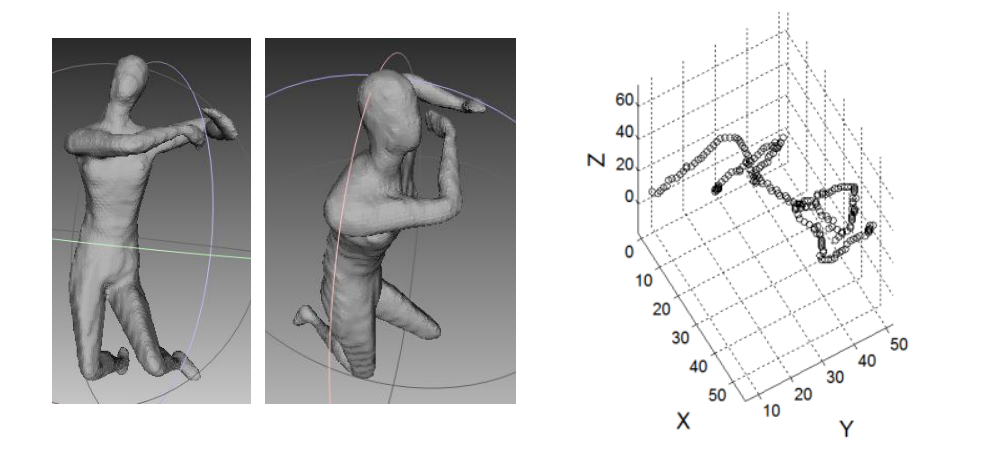
\includegraphics[width=14cm]{content/images/skeletonThinning}
	\caption{Human model and the skeletal representation using the partial parallel \gls{3d} thinning based skeletonizaion algorithm introduced by Jin and Kim \cite{Jin2017}.}
	\label{fig:skeletonThinning}
\end{figure}

A third approach of gathering the skeleton of a \gls{3d} model is presented by Singh and Silver \cite{Singh2004}. They used two approaches one is based on the calculation of the curve skeleton introduced by Gagvani \cite{Gagvani1999} and the other one is based on a potential field algorithm shown by Cornea et.al. \cite{Cornea2005ComputingObjects}. Singh and Silver state that they use both approaches in order to get the \gls{ik} skeleton of the data which does not only consist of the simple skeleton but also has information about bones and joints \cite{Singh2004}. This information is especially important when thinking of interactively transforming data to another position. The positioning of the joints and the bones on the skeleton can be performed manually or semi-automatically. The semi-automatically approach uses the potential field algorithm and the manually one the thinning algorithm. The authors state that the semi-automatically way may be more user-friendly on the other hand the algorithm used in the manual processing is faster \cite{Singh2004}. One major benefit of the algorithm introduced by the authors is that they already automatically calculate the correspondence of each voxel to the specific bone. This is also a huge benefit when thinking of transforming data to a new position. Figure \ref{fig:ikskeleton} represents the data and the corresponding \gls{ik} skeleton.

\begin{figure} [htb!]
    \centering
	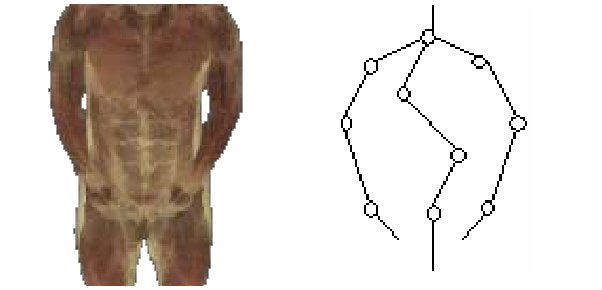
\includegraphics[width=12cm]{content/images/ikskeleton}
	\caption{The given data and the corresponding \gls{ik} skeleton can are figured. The skeleton already features the joints where parts of the volume can be move against \cite{Singh2004}.}
	\label{fig:ikskeleton}
\end{figure}
\newpage

\subsection{Rigging approaches}

Rigging defines the process to determine the skeletal structure and the position of it in a \gls{3d} model in order to be able to move parts of the model and knowing how the surface or the volume has to be deformed \cite{Baran2007}. This task can either be performed in a manually way needing an animator or similar professional to define the skeleton and the position or in an semi-automatic or automatic way. The complexity to automatically rig a \gls{3d} model should not be neglected.

\subsubsection{Pinocchio}
The first approach for automatically rigging a \gls{3d} model represented by its mesh is introduced by Baran and Popovic \cite{Baran2007}. The procedure creates a distance field from the given mesh and it identifies a skeleton by approximating the medial surface. The extracted skeleton is than fitted to template skeleton to refine the output. For their approach they are using discrete penalty functions in order to match the extracted skeleton to a pre defined so called instruction how a skeleton should look like. For example the penalty function checks where the feet are and that they should be on the ground and not at the top area of the mesh. With those penalty functions it can clearly be seen that the method looses generality. The general approach of rigging in the Pinocchio prototype is shown in Figure \ref{fig:pinocchio}.

\begin{figure} [htb!]
    \centering
	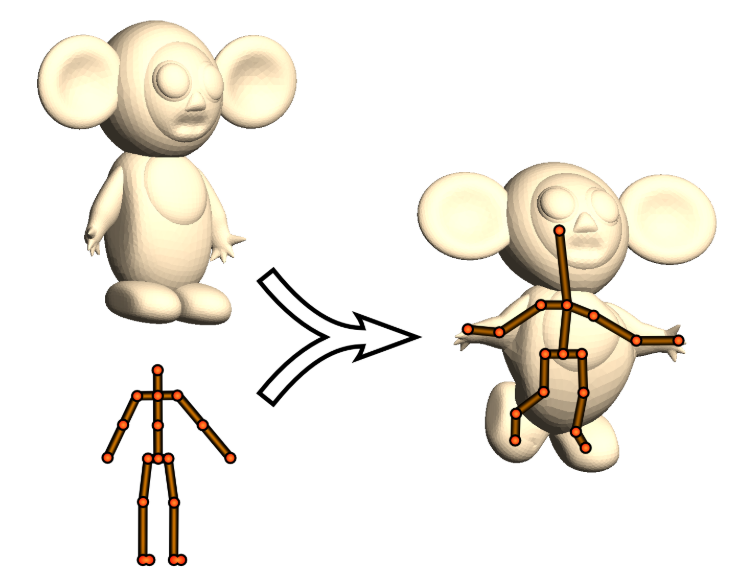
\includegraphics[width=11cm]{content/images/pinocchio}
	\caption{General overview of the pinocchio rigging prototype placing an predefined skeleton into a \gls{3d} mesh model by extracting the curve skeleton and than matching it with a pre-defined prototype skeleton \cite{Baran2007}.}
	\label{fig:pinocchio}
\end{figure}

\newpage
Shapiro et.al. introduce another approach which is quite similar to the strategy of Baran and Popovic but uses voxels instead of the mesh representation of the \gls{3d} model \cite{Shapiro2014RapidSensors}. They have tried to make \gls{3d} scans of humans available for using them in computer animations. Therefore they scanned the humans in four different poses and created a \gls{3d} model out of the gathered data. The difficulty of the rigging was that their mashes where not perfect and had holes and other artefacts. Therefore they decided to create a voxelized version of the mesh by using depth buffer carving. The data they use are produced by the consumer product Kinect \cite{Shapiro2014RapidSensors}. After voxalizing the data they used the same technique as Baran and Popovic \cite{Baran2007} to find the skeleton in the mesh. The approach therefore has the same downside that it does not allow the model to be in another formation before the rigging is done. It has to be in a predefined initial position. The output of the procedure is depicted in Figure \ref{fig:saphiro}.

\begin{figure} [htb!]
    \centering
	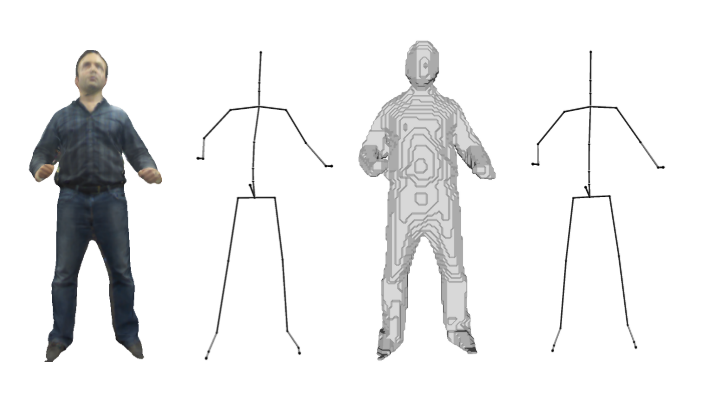
\includegraphics[width=13cm]{content/images/saphiro}
	\caption{On the left the original mesh of the human \gls{3d} scan and the corresponding skeleton. On the right the voxel representation of the mesh using the depth buffers and the skeleton of it. It can be seen that the skeletal representation looks the same for both representations of the \gls{3d} model \cite{Shapiro2014RapidSensors}.} 
	\label{fig:saphiro}
\end{figure}

\subsubsection{Joint mapping}

Bharaj et.al. introduce a procedure which is able to automatically rig a character by using a joint mapping technique \cite{Bharaj2012}. Their approach is especially suitable for multi component characters. They are using point clouds in order to sample each identified component of the input model. These clouds are represented as a a graph which is simplified and transformed into a tree by using clustering. Their attempt needs as a second input an animation skeleton which is predefined. The authors use joint mapping in order to find the relation between their tree and the given animation skeleton. Normally the mapping is defined by a user. Their approach is closely related to the approach stated in this thesis because they also would like to afterwards find a way to transform the data into a standardized T-pose \cite{Bharaj2012}. The transformation of the data can be done using an animation software because their export format is an industrial standard. Two examples of their rigging process can be seen having a look at Figure \ref{fig:bharaj}.

\begin{figure} [htb!]
    \centering
	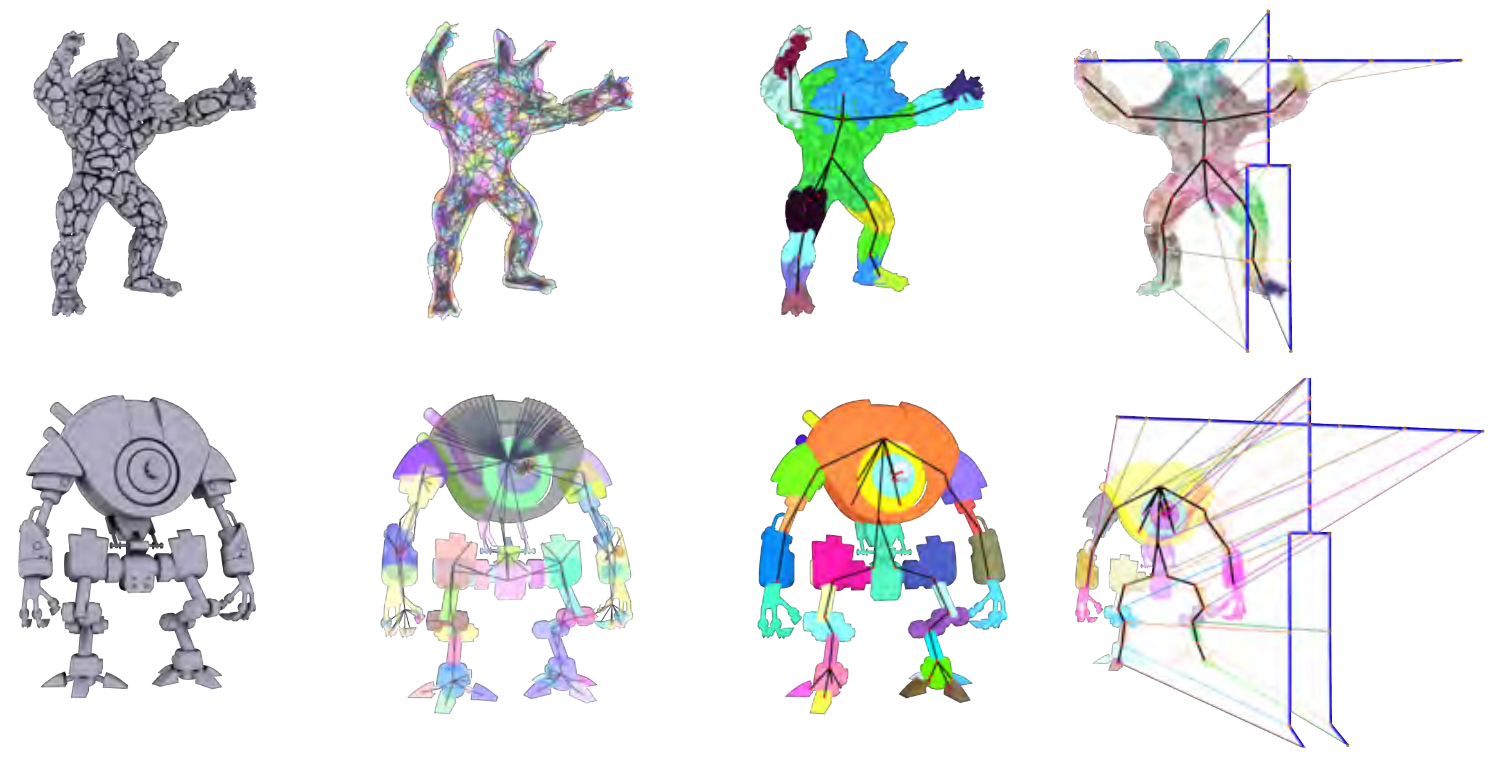
\includegraphics[width=15cm]{content/images/baharaj}
	\caption{Two multi component models rigged by the approach of Bharaj et.al.  \cite{Bharaj2012}.} 
	\label{fig:bharaj}
\end{figure}

\subsubsection{Manual rigging}

Manual rigging is the process to define the position of a predefined skeleton or armature in a mesh or volume. The user has to first define the skeleton and than to drag the joints and the bones into the model in order to define the rigging of it. Finet et.al. introduced a software called Bender which is open source software used for efficient model posing and morphing \cite{Finet2014Bender:Morphing}. One of their modules is called Armatures and enables the user to rig a model by defining or loading an armature in the *.vtk format and afterwards also saving the result. The armature can be represented in different ways using lines, cylinders or octohedrons. The armature parts are defined from a head to a tail. The head is normally connected to another armature part unless it is the first one. The tail may not be connected e.g. in case of the feet or the hands. The armature created has a hierarchy which can be defined individually. Each part of the armature can have a name. An example armature and the software are shown in Figure \ref{fig:Armatures}.

\begin{figure} [htb!]
    \centering
	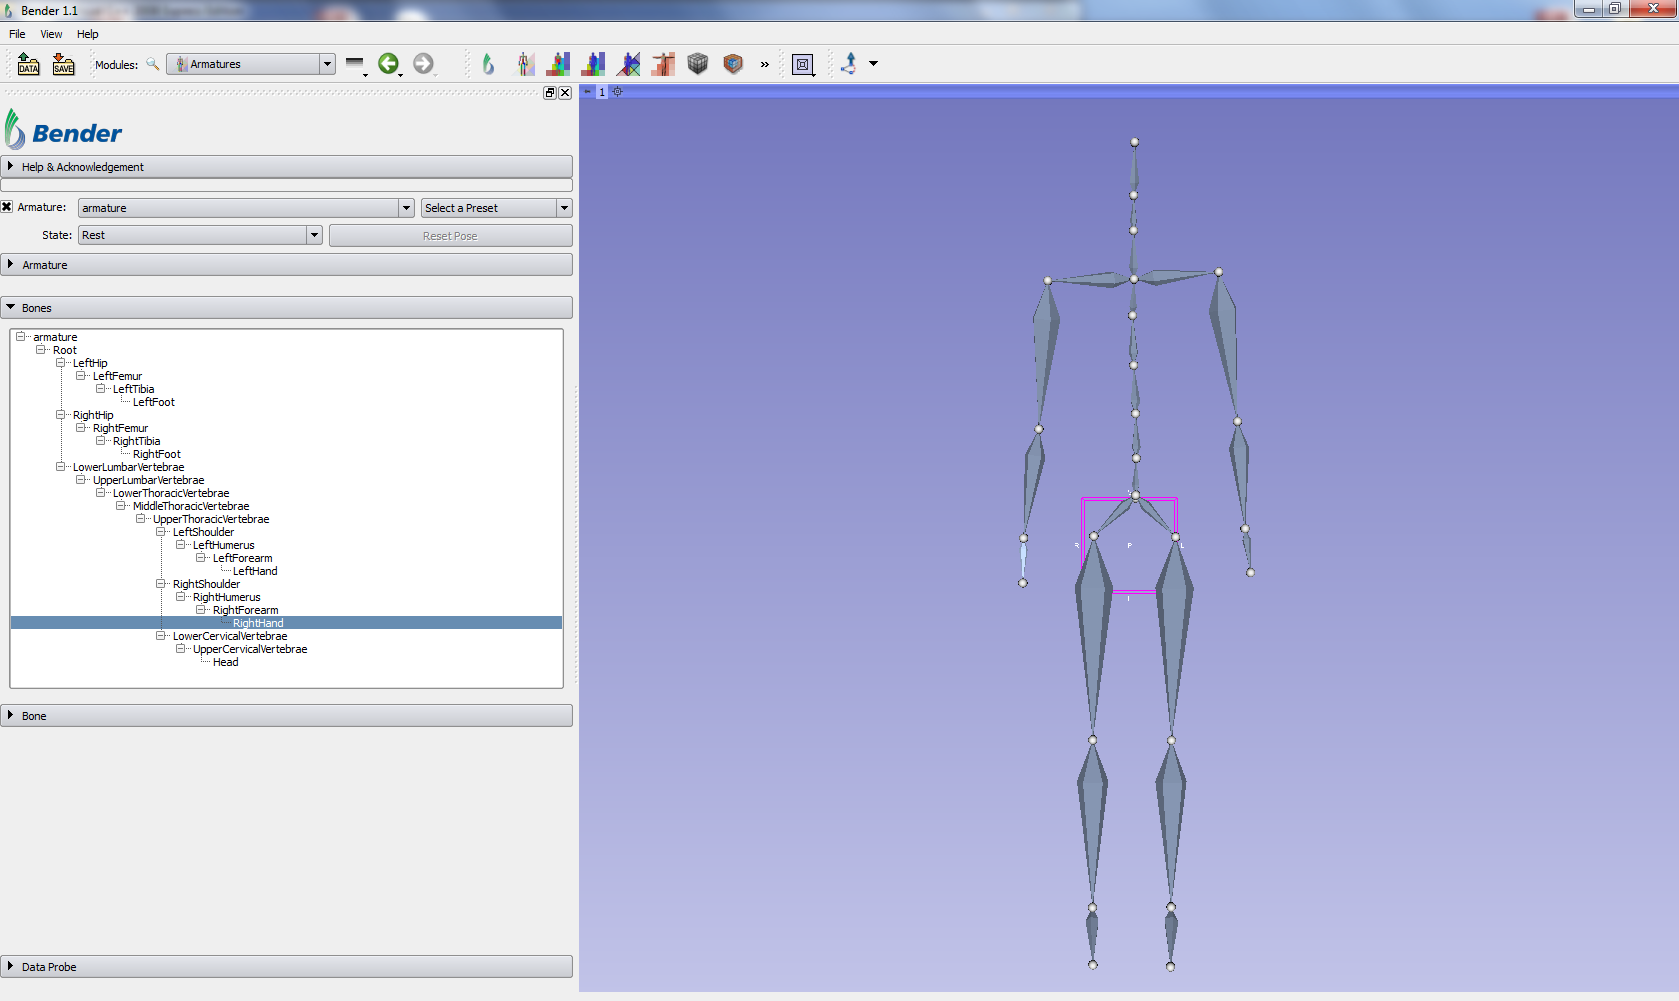
\includegraphics[width=14cm]{content/images/Armatures}
	\caption{Screenshot of the armature module of Bender. The shown armature is only en example and can be individually customized and generated. The screen is also used to drag the armature into the model if a model is loaded \cite{Andruejol2014BenderModules}.} 
	\label{fig:Armatures}
\end{figure}

\newpage
\section{Skinning or weighting of the armature}

After the armature or the skeleton is defined and the position inside of the mesh or volume has been found the data has to be weighted. That means that either the mesh or the voxels have to be linked to parts of the armature in order to know which parts have to be moved or transformed to create an animation or simply a movement. Some rigging approaches which originate from skinning the data already have this information available because during the skinning process the program simply has to save which voxels have to be removed in order to create parts of the skeleton. Afterwards these voxels are those who belong to the specific parts of the armature. One approach that is well known and has been introduced by Magnenat-Thalmann et.al. is called \gls{lbs}. The principal behind the algorithm is that between two adjacent points of the armature there can be a so called heat distributed plotted. This distribution can be used in order to define which mesh or voxel parts are deformed or affected by a movement of the given segment. Figure \ref{fig:lbs} visualizes how the \gls{lbs} works.

\begin{figure} [htb!]
    \centering
	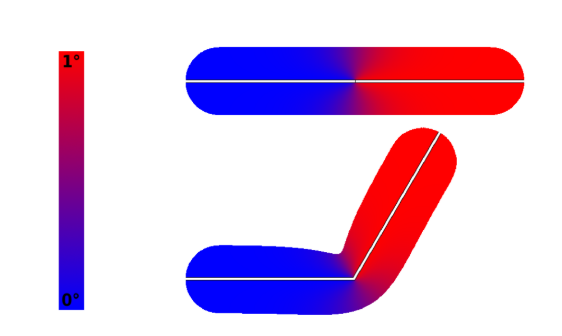
\includegraphics[width=10cm]{content/images/lbs}
	\caption{The left side of the image represents the heat distribution between two points which can also be seen at the top. The lower parts shows how the e.g. voxels will be affected if the right part of the joint moves about 45 degrees \cite{Baran2007}.} 
	\label{fig:lbs}
\end{figure}

\newpage

In case of the topological approach introduced by \cite{Bharaj2012} the skinning is already available because it is well known how the data have been abstracted in order to generate the point cloud, the graph and at the end the tree. The skinning of their approach also conforms the \gls{lbs} approach. The Pinocchio prototype uses the \gls{lbs} method to calculate for each vertex of the mesh the weight how it is affected by a bone transform. It is stated that it is highly affected by the distance to the bone and the interaction between two bones is calculated by using the \gls{lbs} method \cite{Baran2007}.

\subsection{Geodesic voxel binding}

Dionne and Lasa introduced the geodesic voxel binding as a voxel weighting approach in order to be able to transform voxel based characters using an armature \cite{Dionne2013GeodesicMeshes}. The authors state that their approach is particularly useful when having data that is not represented by a watertight mesh. They use the geodesic distance between each voxel and the nearest bone from the skeleton in order to determine which voxel is affected by which bone. The benefit is that the mash does not have to perfect and the complexity of the calculation is low and therefore fast \cite{Dionne2013GeodesicMeshes}. The process described by the authors is shown in Figure \ref{fig:geodesic}.

\begin{figure} [htb!]
    \centering
	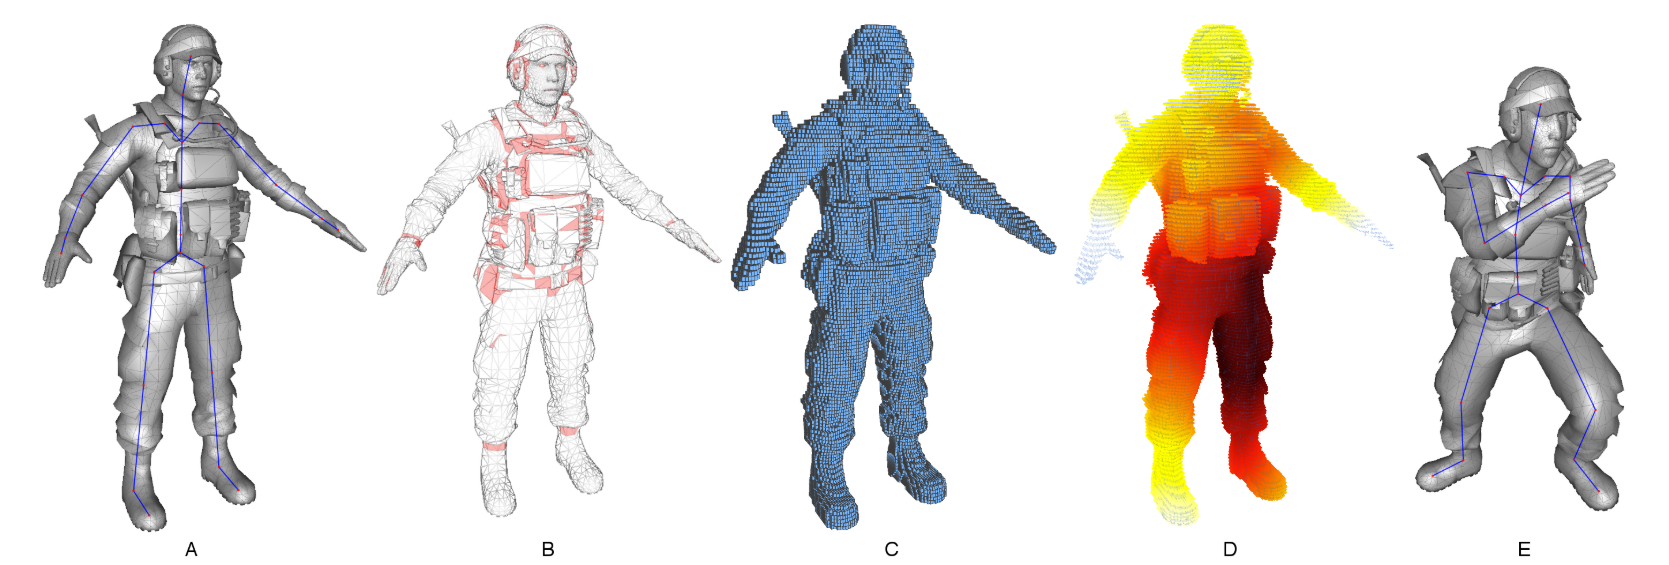
\includegraphics[width=13cm]{content/images/geodesic}
	\caption{This image represents the whole processing pipeline from the mesh at the beginning over the voxelized model in the middle, the geodesic representation at position D and the transformed mesh at the right hand side. Position B represents that there are some imperfections in the mesh which make it not watertight and therefore unsuitable for different skinning approaches \cite{Dionne2013GeodesicMeshes}.} 
	\label{fig:geodesic}
\end{figure}

\newpage

\subsubsection{Bender VolumeSkinning}

Bender has a volume skinning module which takes the volume as an input and an predefined armature \cite{Finet2014Bender:Morphing}. It then calculates the weights an delivers as output a new volume where the voxels are identified by the IDs of the armature parts they belong to. The mapping between armature parts and the voxels belonging to it are represented using different colors. One example output of the bender software is shown in Figure \ref{fig:BenderVolumeSkinning}.

\begin{figure} [htb!]
    \centering
	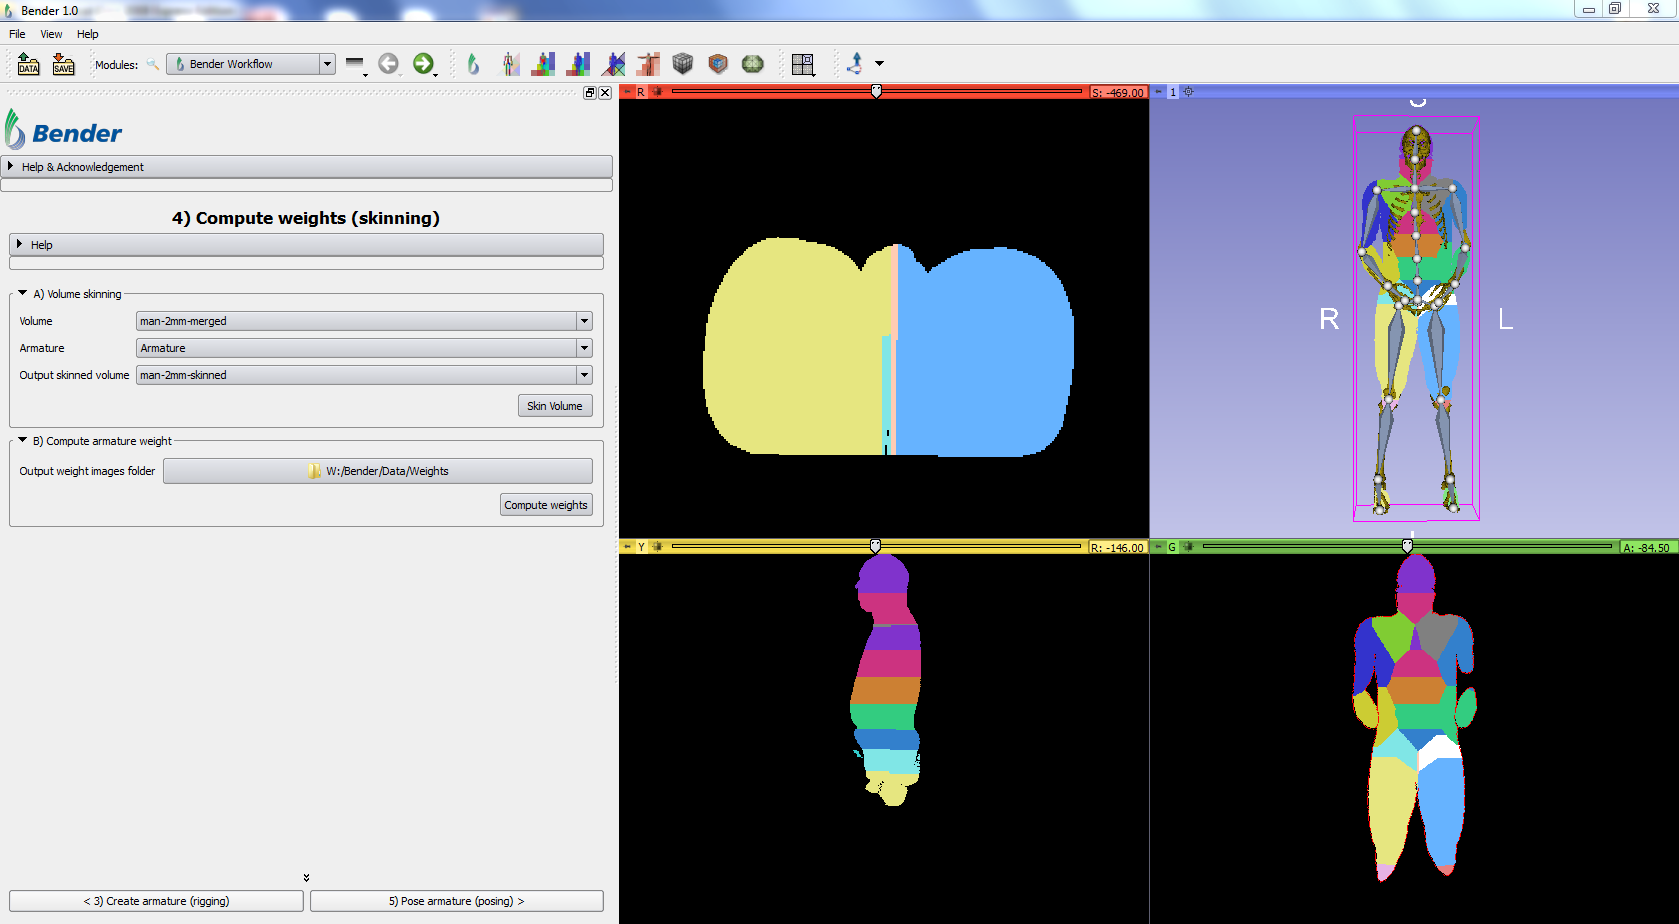
\includegraphics[width=13cm]{content/images/BenderVolumeSkinning}
	\caption{The Bender VolumeSkinning module with an example output of the armature and the skinned volume depicted in different colors representing which parts of the model belong to which armature part \cite{Andruejol2014BenderModules}.} 
	\label{fig:BenderVolumeSkinning}
\end{figure}

\section{Reformation of volumetric data}

The reformation of volumetric data can be performed in different ways. Some possibilities are shown in this sections.

\subsection{VolEdit}

Singh and Silver have introduced a method to manipulate volumetric data by using the \gls{ik} skeleton \cite{Singh2004}. After having identified the skeleton in the data and the joints of the skeleton they can use their software to manipulate the volume. One approach is to transform the skeleton using rotations around a joint. They are able to move each segment of the skeleton individually in respect to the according joint. In their approach the authors are using a program called VolEdit to modify the volumetric data \cite{Singh2004}. A simple interaction can be to apply a  transfer function to different parts of a model and to combine them. Figure \ref{fig:lobster} represents a lobster model which has been transformed using two different transfer functions in order to move the arms of the animal away from the body.

\begin{figure} [htb!]
    \centering
	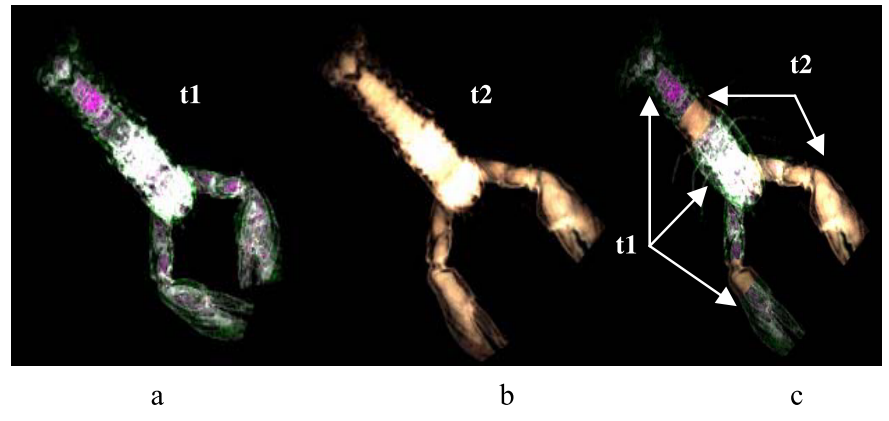
\includegraphics[width=13cm]{content/images/lobster}
	\caption{The lobster model transformed with two different transfer function which are applied to different regions of the model in order to move the arms away from the body \cite{Singh2004}.} 
	\label{fig:lobster}
\end{figure}

Using the same software VolEdit the authors also showed another example where they tried to unbend a rat which has been pictured in a small housing. This technique can be used to bring pictures into a standardized form like used in this thesis \cite{D.SilverK.yawsC.CorreaW.HurtP.Mason2005VolumetricSimulations}. Figure \ref{fig:mouse} shows the rat example before and after the unbending. Another interesting approach of Singh and Silver is to do a so called juxtaposition of different data sets. Using their program they are able to exchange the arm of a man by the arm of a lobster and the result looks quite promising. The application of the juxtaposition is depicted in Figure \ref{fig:juxtaposition}.

\begin{figure}
    \centering
	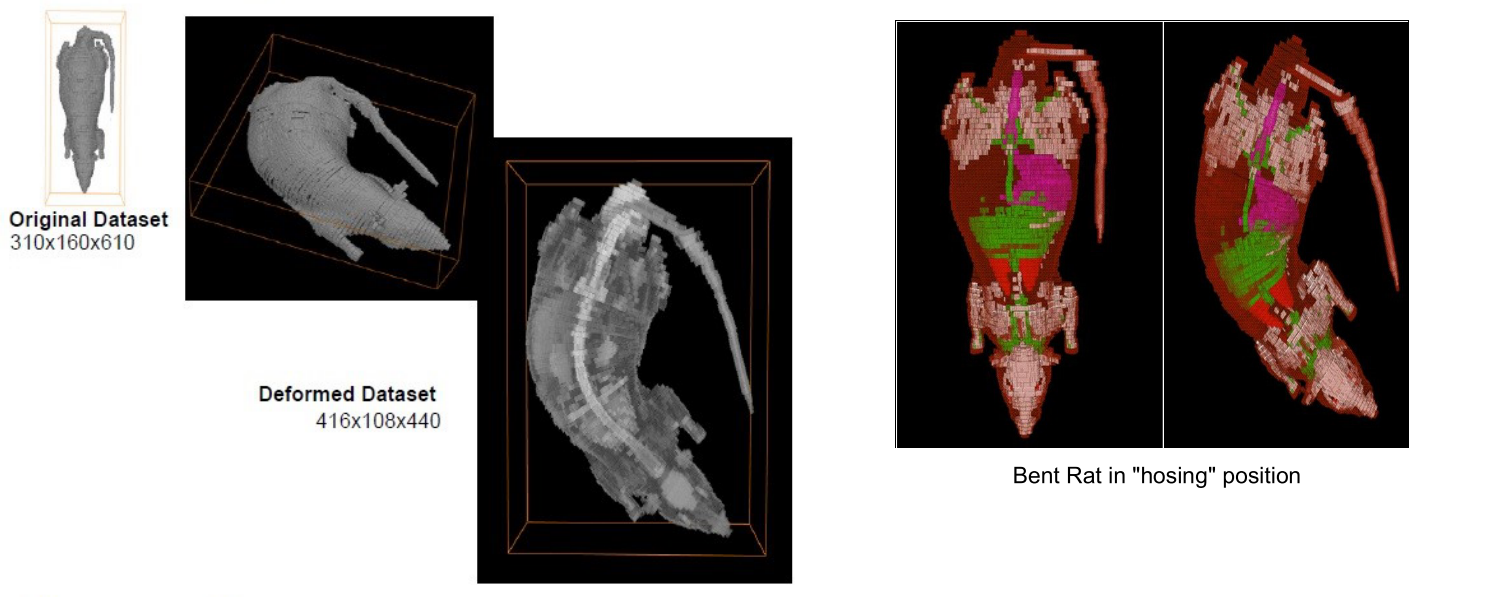
\includegraphics[width=13cm]{content/images/mouse}
	\caption{Unbending of a rat which is capt in a small housing \cite{D.SilverK.yawsC.CorreaW.HurtP.Mason2005VolumetricSimulations}.} 
	\label{fig:mouse}
\end{figure}

\begin{figure}
    \centering
	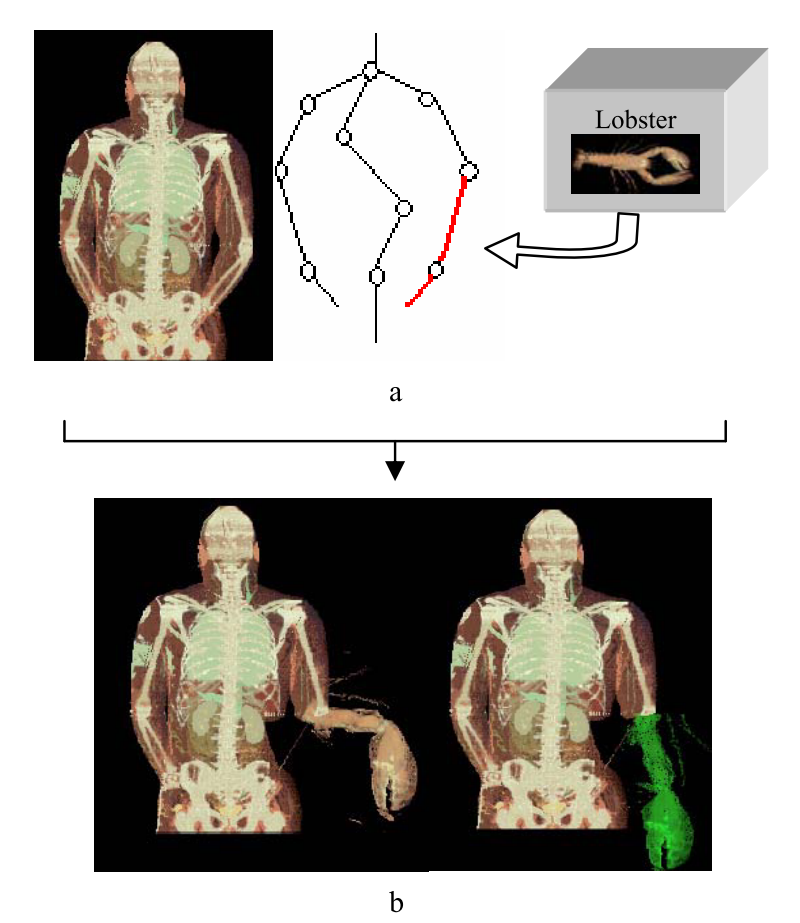
\includegraphics[width=10cm]{content/images/juxtaposition}
	\caption{Juxtaposition of the arm of a man and the arm of a lobster \cite{Singh2004}.} 
	\label{fig:juxtaposition}
\end{figure}

\subsection{Volume manipulation for surgical processes}

Nakao and Minato represent in their paper a novel techniques which can be used by surgeons to prepare for their surgical process or to share their knowledge in an interactive and visual appealing way \cite{Nakao2010}. In their application the user is able to manipulate patient specific volumetric data according to a real surgical intervention. The authors used \gls{ct} and \gls{mri} images as a source for their method and enable the user to perform physically correct modelled surgical procedures. The used a vertices based grid and finite element analysis in order to create a visualization that behaves physical correctly \cite{Nakao2010}.  An example for such a surgical intervention and the volumetric rendering can be seen in Figure \ref{fig:physical}.

\begin{figure} [htb!]
    \centering
	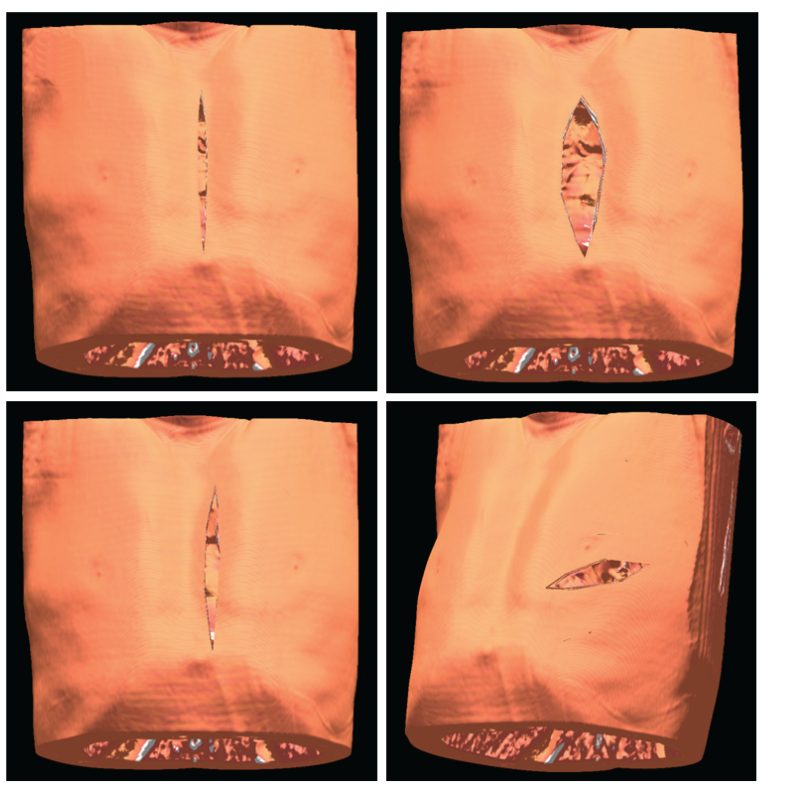
\includegraphics[width=11cm]{content/images/physical}
	\caption{Visualization of a volume cutting considering the tension that arises from the surrounding tissue resulting in a cleft with a differing size \cite{Nakao2010}.} 
	\label{fig:physical}
\end{figure}